\subsection{Qualitative Evaluation: Clustering}

\begin{itemize}
\item Mention again how the feature vectors are extracted
\item What questions we want to answer here
\item Comparison against baseline to show that results are not random
\end{itemize}

\begin{figure}[htb]
\centering
  \begin{subfigure}[b]{.24\linewidth}
    \centering
    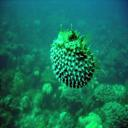
\includegraphics[width=.99\textwidth]{figures/clustering/aquarium}
    \caption{input image}\label{fig:clustering_aquarium_input}
  \end{subfigure}  \\%
  \begin{subfigure}[b]{.99\linewidth}
    \centering
    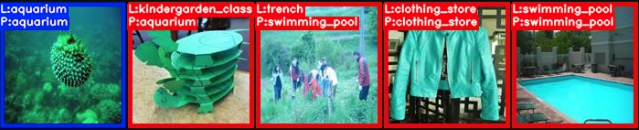
\includegraphics[width=.99\textwidth]{figures/clustering/aquarium_conv1_avg}
    \caption{conv1 cluster}\label{fig:clustering_aquarium_conv1}
  \end{subfigure}  \\%
  \begin{subfigure}[b]{.99\linewidth}
    \centering
    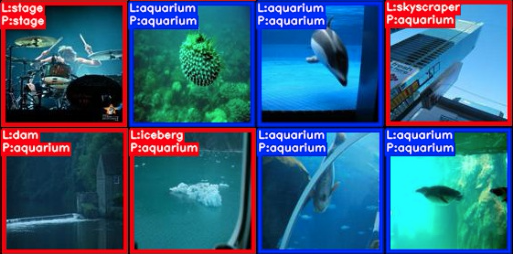
\includegraphics[width=.99\textwidth]{figures/clustering/aquarium_conv4_avg}
    \caption{conv4 cluster}\label{fig:clustering_aquarium_conv1}
  \end{subfigure}  \\%
  \begin{subfigure}[b]{.99\linewidth}
    \centering
    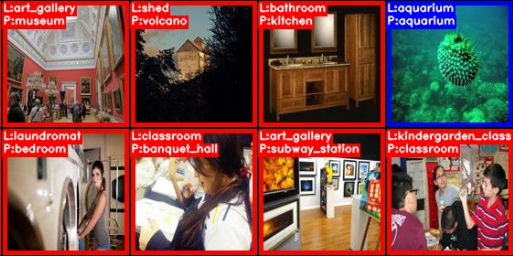
\includegraphics[width=.99\textwidth]{figures/clustering/aquarium_dhash}
    \caption{perceptual image hashing cluster (baseline)}\label{fig:clustering_baseline}
  \end{subfigure}%
  \caption{Example clusters obtained for an input aquarium image from MiniPlaces dataset.}
  \label{fig:aquarium_clusters}
\end{figure}